\documentclass[openany, twoside, a4paper, 12pt]{extbook}
\usepackage{amsmath}
\usepackage{amsfonts}
\usepackage{geometry}
\usepackage[russian]{babel}
\usepackage{fancyhdr}
\usepackage{titlesec}
\usepackage{indentfirst}
\usepackage{lipsum}
\usepackage{graphicx}

% Устанавливаем поля страницы
\geometry{a4paper, margin=1in}
\setlength{\headheight}{15pt}
% Отключаем нумерацию на титульном листе
\pagenumbering{gobble}

% Настройка стиля страницы после титульного листа
\fancypagestyle{mystyle}{
    \fancyhf{} % очищаем текущие значения
    \fancyhead[L]{\thepage} % Номер страницы слева сверху
    \renewcommand{\headrulewidth}{0pt} % убираем линию
}

\begin{document}

\title{\textbf{Формальная постановка задачи оптимизации расписания с использованием алгоритма имитации отжига}}
\author{Варгин Артём Анатольевич}
\date{\today}
\maketitle

% Включаем нумерацию страниц после титульного листа
\newpage
\pagenumbering{arabic}
\pagestyle{mystyle}

\section*{Формальная постановка задачи}

    \subsection*{Дано:}
        \begin{itemize}
            \item  $N$ --  количество работ;
            \item $J = \{j_1, j_2, \dots, j_N\}$ -- множество работ;
            \item $\tau  = \{t_1, t_2, \dots, t_N\}$ -- множество времен выполнения соответстующих заданий $j_i$, $\forall i \in \overline{1,N}$ $t_i > 0$.
            \item  $M$ --  количество процессоров;
            \item $P = \{p_1, p_2, \dots, p_M\}$ -- множество процессоров, на которых выполняются работы.
        \end{itemize}
    
    \subsection*{Расписание:}
        Расписанием является булева матрица $HP \in B^{N \times M}$, в которой $hp_{ij} \in \{0, 1\}$, где $i \in \overline{1, N}$, а $j \in \overline{1,  M}$. Значение $s_{ij} = 1$ означает,
        что работа с номером $i$ выполняется на процессоре с номером $j$, а $hp_{ij} = 0$ -- что работа с номером $i$ не выполняется на процессоре с номером $j$.
        

    \subsection*{Требуется:}
        Построить расписание $HP^{N \times M}$, при котором будет минизирован критерий, при этом все задания $J$ будут выполнены на множестве процессоров $P$ без прерываний,
        с учетом ограниченных ресурсов, и не будет пересечений в использовании процессоров, т.е.

        $\forall i \in \overline{1, N}$ $ \exists! j \in \overline{1, M}:$ $hp_{ij} = 1$ $\Leftrightarrow$

        \begin{equation*}
         \begin{cases}
           $\sum\limits_{i=1}^N \sum\limits_{j=1}^M hp_{ij} = N$
           \\
            $\forall i \in \overline{1, N} \sum\limits_{j=1}^M hp_{ij} = 1$
         \end{cases}
        \end{equation*}

    \subsection*{Минимизируемый критерий:}
        В зависимости от остатка от деления на 2 контрольной суммы CRC32 от фамилии и инициалов выбирается один из следующих критериев:
        \begin{itemize}
            \item Критерий $K_1$ (разбалансированность расписания)
            \item Критерий $K_2$ (суммарное время ожидания)
        \end{itemize}
        
        $CRC32_{ВаргинАА} = 42570633$, следовательно выбираем 1 критерий для реализации.

        \subsubsection*{Критерий разбалансированности расписания:}
        Обозначим $G_j$ - упорядоченное по последовательности выполнения множество индексов работ, которые выполняются $j$-ым процессором. Тогда 
        $T_j = \Sigma_{i \in G_j}t_i$ -- суммароное время выполнения работ, запланированных на $j$-ый процессор.

        \begin{equation}
            K_1 = T_{max} - T_{min}
        \end{equation}
        где:
        \begin{equation}
            T_{max}= \max_{j \in \overline{1,  M}}T_j
        \end{equation}
        \begin{equation}
            T_{min} = \min_{j \in \overline{1,  M}}t_{G_j[0]}
        \end{equation}
        
\section*{Ограничения}

    \begin{itemize}
        \item Каждый процессор $p_j \in P$ в любой момент времени может выполнять не более одного задания.
        \item Во время выполнения задания процессором, не возникает прерываний.
        \item Процессор может мгновенно (без прерывания) переключаться между заданиями.

        \item Время выполнения $t_i \in \tau$ фиксировано.
    \end{itemize}
\newpage
\section*{Исследование последовательного алгоритма}
\begin{figure}[ht]
    \centering
    \begin{minipage}{0.49\textwidth}
        \centering
        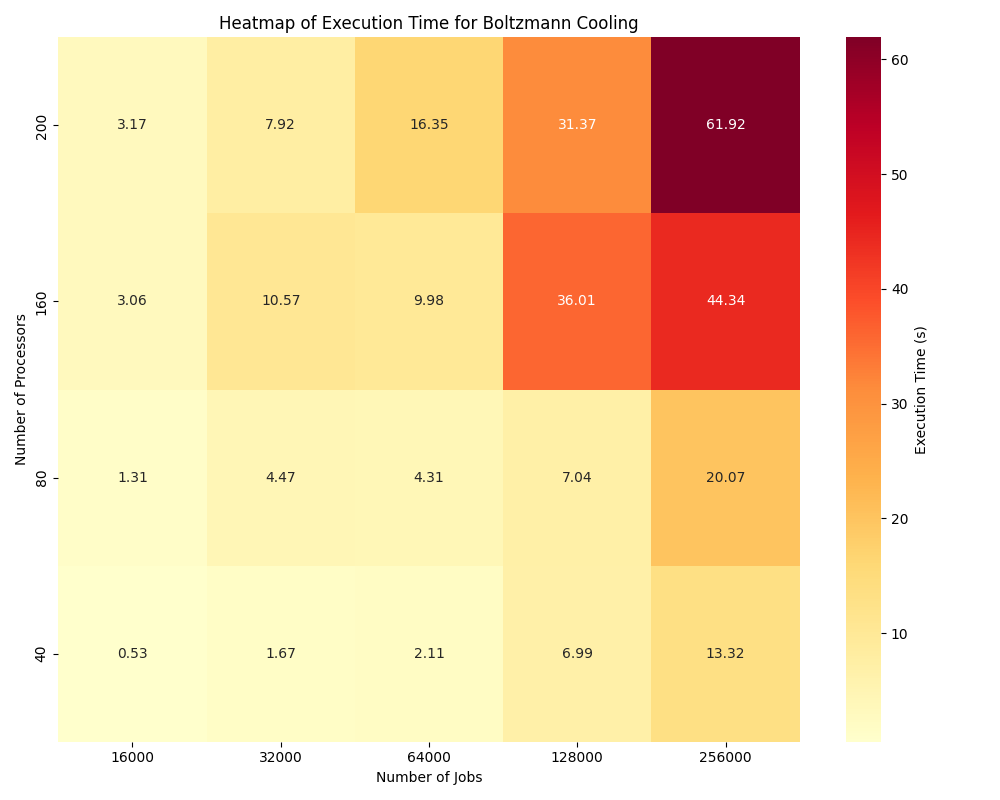
\includegraphics[width=\textwidth]{results_solo/boltzmann_cooling_heatmap_execution_time.png}
        %\caption{Время выполнения алгоритма с охлаждением Больцмана}
        \label{fig:image1}
    \end{minipage}
    \hfill
    \begin{minipage}{0.49\textwidth}
        \centering
        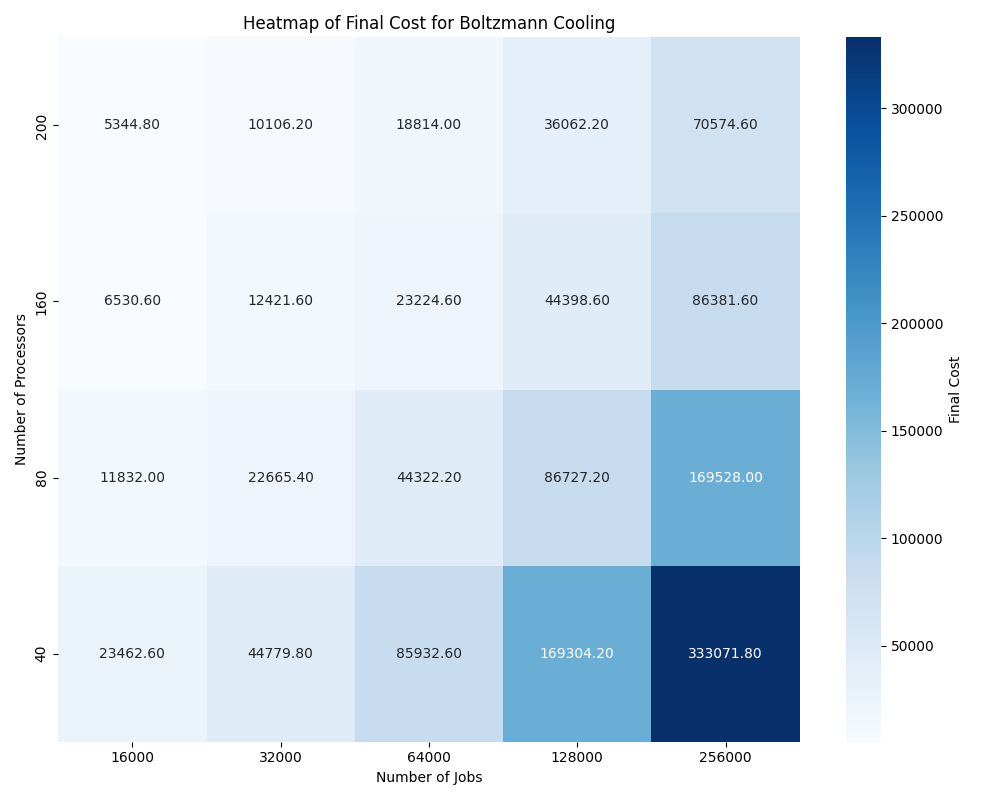
\includegraphics[width=\textwidth]{results_solo/boltzmann_cooling_heatmap_final_cost.png}
        %\caption{Значения метрик алгоритма Болцмана}
        \label{fig:image2}
    \end{minipage}
    \vspace{-50pt} % Уменьшаем пространство между блоками
\end{figure}

\begin{figure}[ht]
    \centering
    \begin{minipage}{0.49\textwidth}
        \centering
        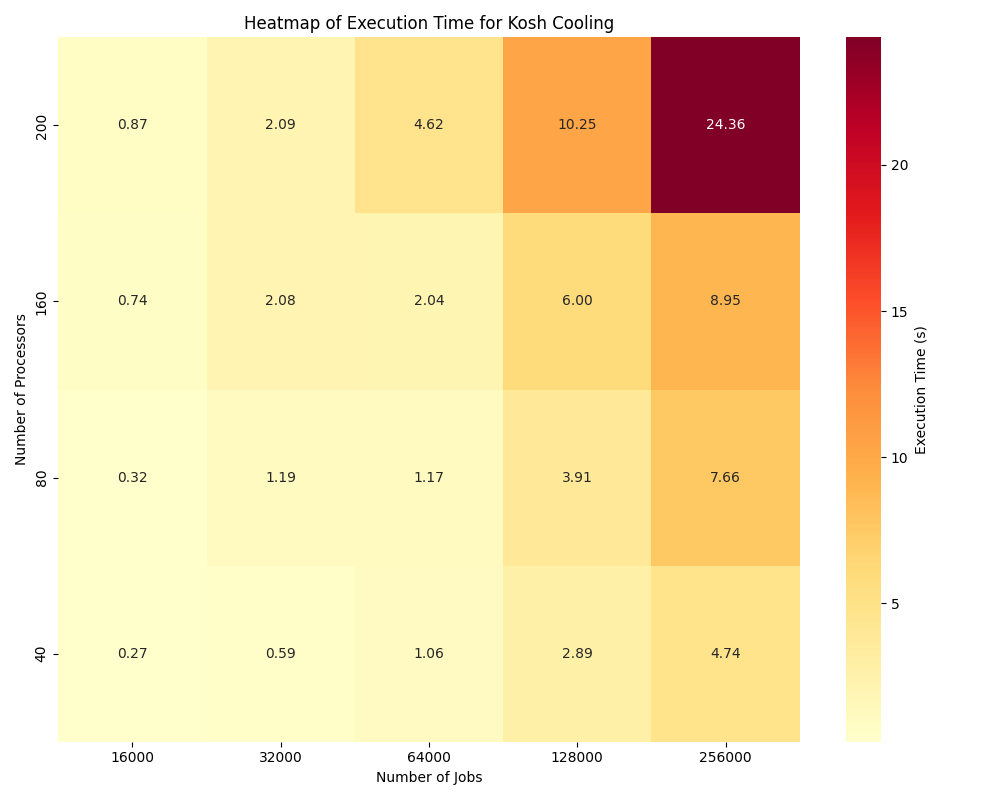
\includegraphics[width=\textwidth]{results_solo/kosh_cooling_heatmap_execution_time.png}
        %\caption{Время выполнения алгоритма с охлаждением Коши}
        \label{fig:image3}
    \end{minipage}
    \hfill
    \begin{minipage}{0.49\textwidth}
        \centering
        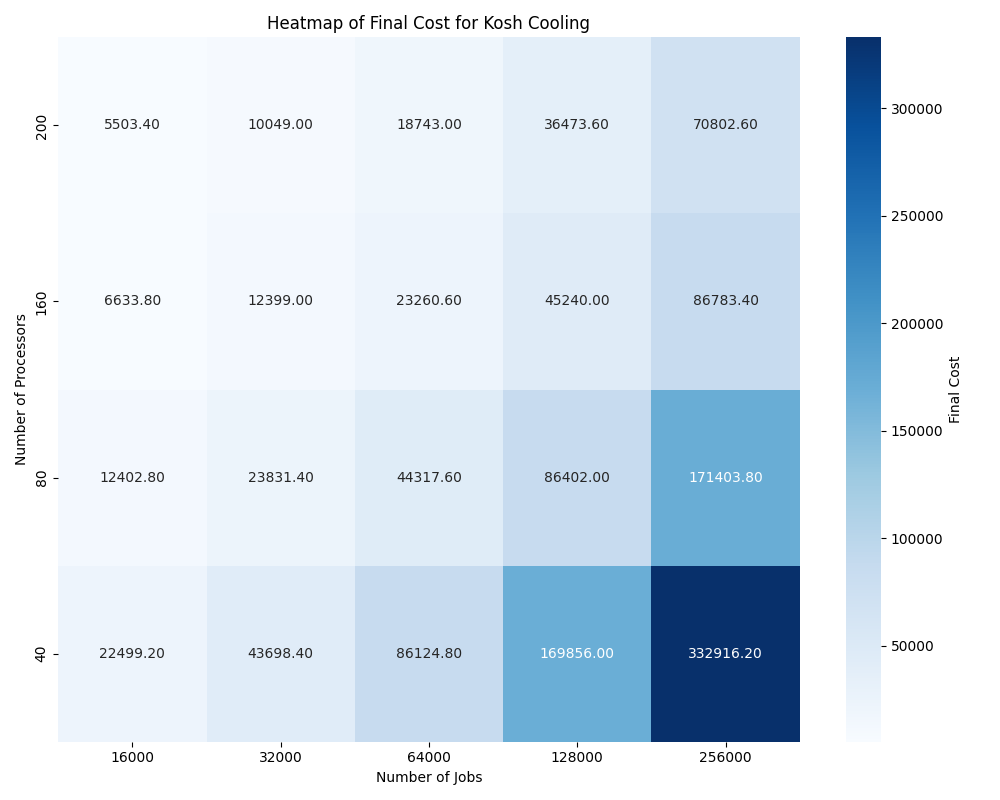
\includegraphics[width=\textwidth]{results_solo/kosh_cooling_heatmap_final_cost.png}
        %\caption{Значения метрик алгоритма Коши}
        \label{fig:image4}
    \end{minipage}
    \vspace{-50pt} % Уменьшаем пространство между блоками
\end{figure}

\begin{figure}[ht]
    \centering
    \begin{minipage}{0.49\textwidth}
        \centering
        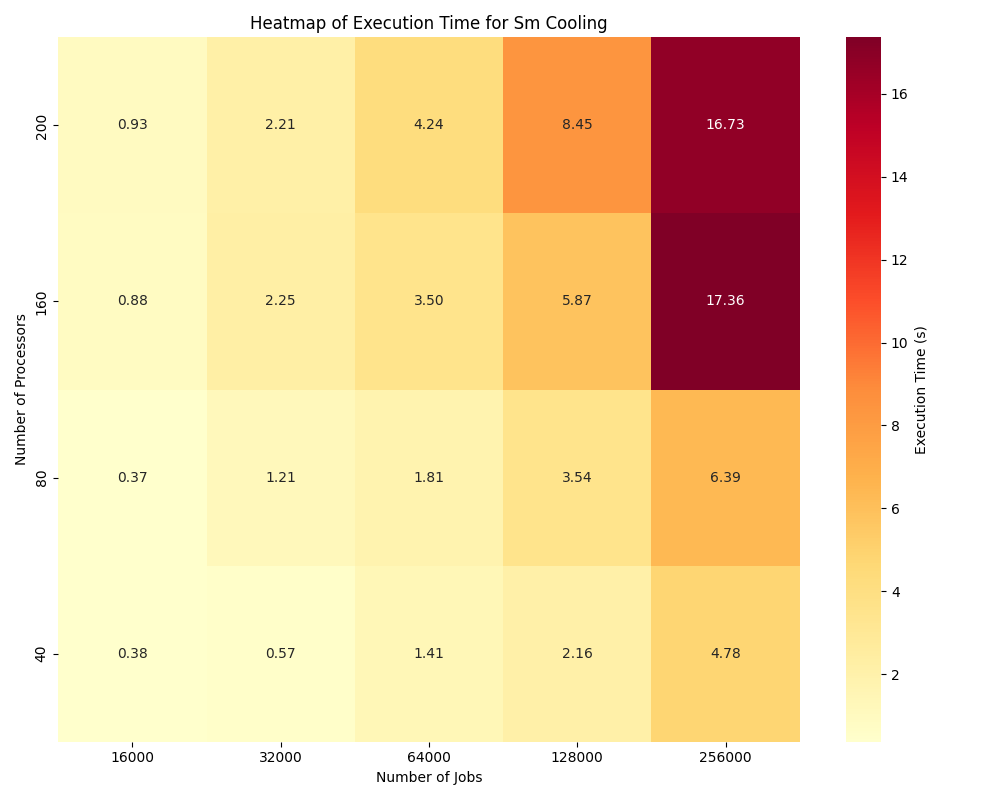
\includegraphics[width=\textwidth]{results_solo/SM_cooling_heatmap_execution_time.png}
        %\caption{Время выполнения алгоритма с логарифмическим охлаждением}
        \label{fig:image5}
    \end{minipage}
    \hfill
    \begin{minipage}{0.49\textwidth}
        \centering
        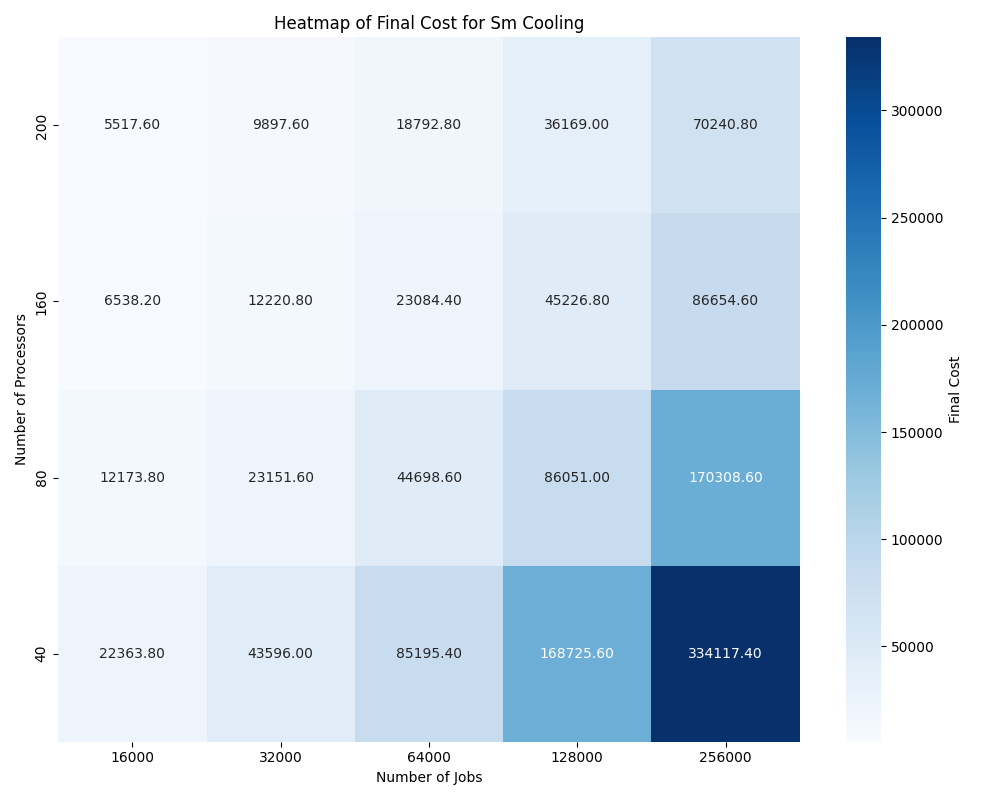
\includegraphics[width=\textwidth]{results_solo/SM_cooling_heatmap_final_cost.png}
        %\caption{Значения метрик алгоритма с логарифмическим охлаждением}
        \label{fig:image6}
    \end{minipage}
    %\vspace{-50pt} % Уменьшаем пространство между блоками
\end{figure}

Представленные значения получены усреднением 5 запусков последовательного алгоритма имитации отжига.

На основании проведенных исследований можно сделать вывод, что алгоритм понижения температуры на основе модели Больцмана демонстрировал самое длительное время выполнения по сравнению с другими алгоритмами (потому что этот закон понижения температуры самый медленный). Тем не менее, это не отразилось на точности вычислений. Все алгоритмы показали сопоставимые результаты.

\newpage
\section*{Исследование параллельного алгоритма}
\begin{figure}[h]
    \centering
    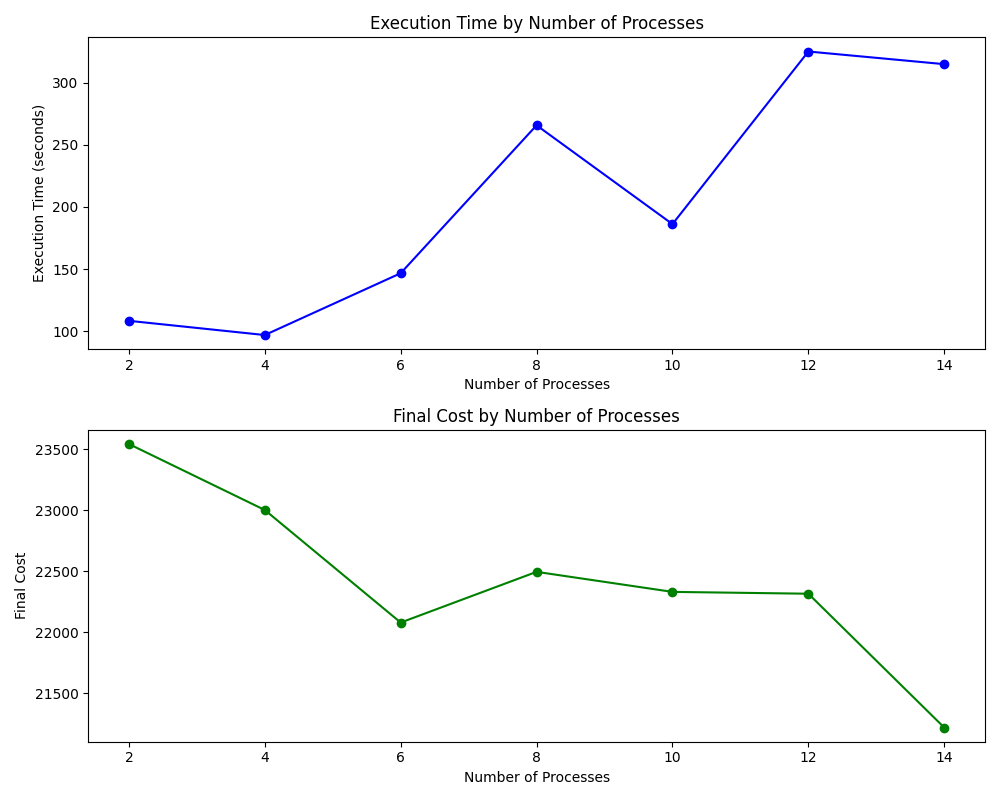
\includegraphics[width=0.8\textwidth]{metrics_plot.png}
    %\caption{Описание изображения 2}
    \label{fig:image7}
\end{figure}

В графе представлены средние значения метрик за 5 запусков, были взяты данные из 16000 задач и 40 процессоров. На основе полученных данных можно понять, что параллельный алгоритм работает многократно дольше последовательной версии, однако имеет прирост производительности.
\end{document}